\begin{figure}
  \centering
  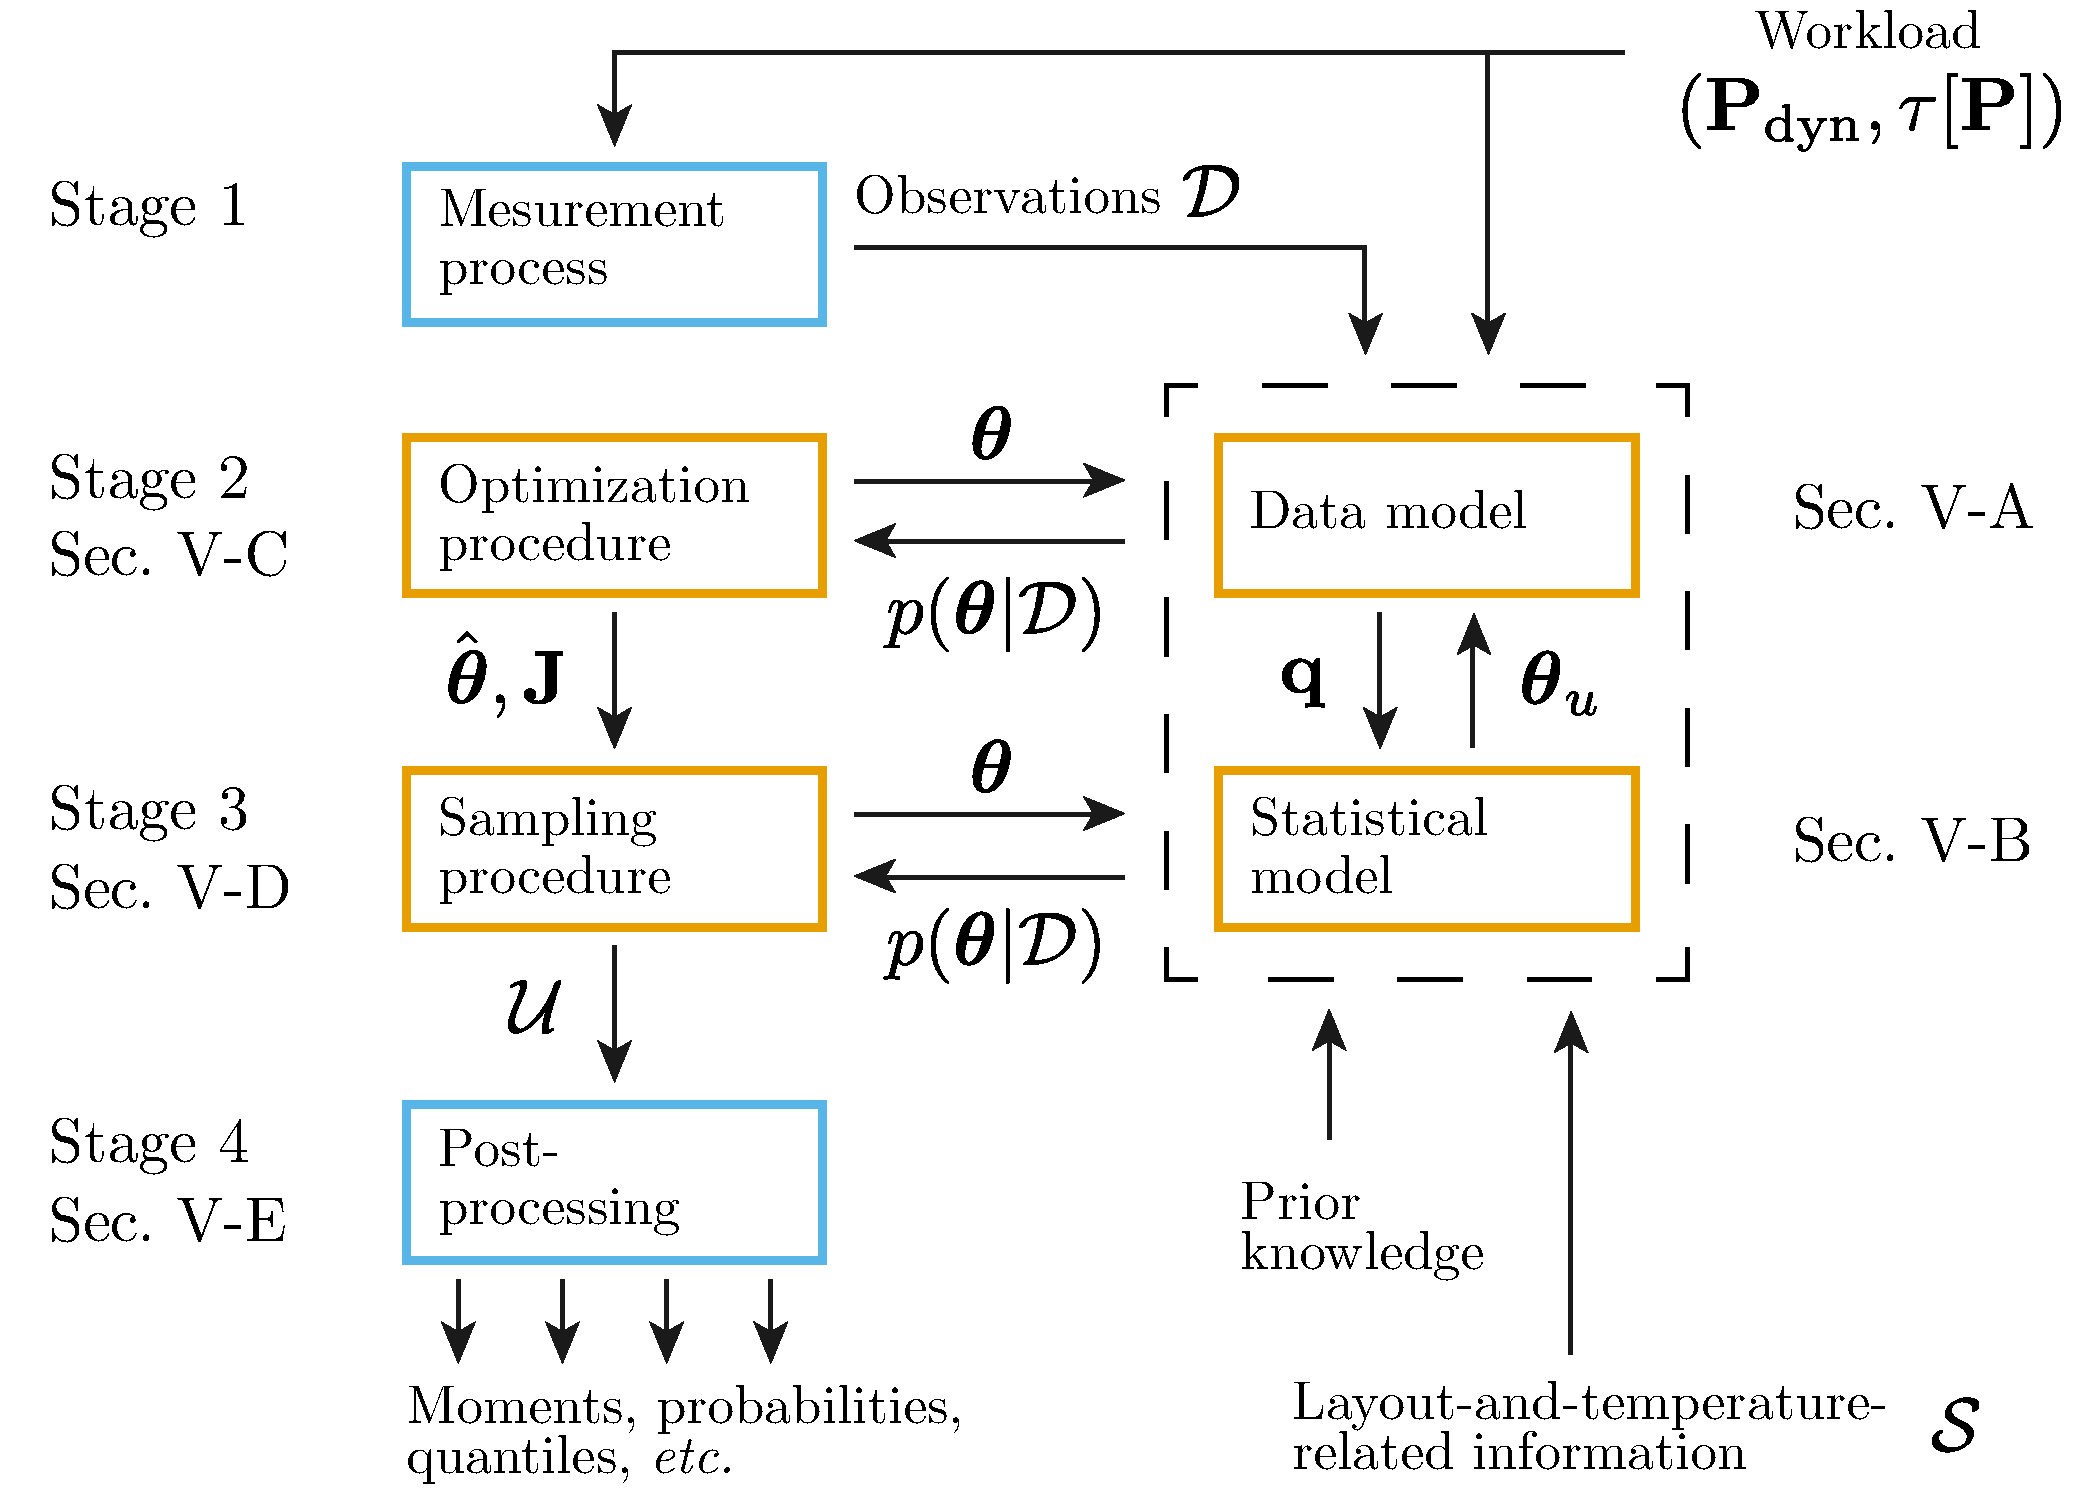
\includegraphics[width=0.80\linewidth]{include/figures/algorithm.pdf}
  \caption{The proposed framework.}
  \flabel{algorithm}
\end{figure}

In this section, we present our temperature-based technique for the characterization of process variation. The framework is divided into four major stages depicted in \fref{algorithm}.
Stage~1 is the data-harvesting stage wherein the user is supposed to collect a set of observations $\Data$ as described in \sref{motivation}.
At Stage~2, we undertake an auxiliary procedure that delivers an optimized proposal distribution to the MCMC sampling in Stage~3.
Stage~3 produces a collection of samples of the \qoi, such as the effective channel length, which is then processed at Stage~4 in order to estimate various characteristics, specified by the user, of this \qoi, \eg, to compute the probability of the effective channel length to be smaller than a certain threshold as motivated in \sref{motivation}.
As it can be seen in \fref{algorithm}, Stage~2 and Stage~3 actively communicate with two models on the right, called the data and statistical models, which we shall discuss next.

\subsection{Data Model} \slabel{data-model} \slabel{power-model} \slabel{thermal-model}
The total power of a system with $\ncores$ processing elements at time $\t$ is composed of the dynamic and leakage parts:
\begin{equation} \elabel{total-power}
  \vP(\t, \vT(\t), \u) = \vP_\dyn(\t) + \vP_\leak(\vT(\t), \u)
\end{equation}
where $\vP, \vT \in \real^\ncores$ are vectors of power and temperature, respectively, and $\u$ is an outcome of the parametrization $\U$. The dynamic part, $\vP_\dyn$, is temperature-independent whereas the leakage part, $\vP_\leak$, is a strong function of the operating temperature. The influence of process variation on the dynamic power is known to be negligibly small \cite{srivastava2010}; therefore, only leakage is assumed to be dependent on $\U$.


Given the thermal specification $\specification$ (see \sref{problem-formulation}) of the multiprocessor system at hand, an equivalent representation, capturing the thermal behavior of the system, can be constructed \cite{kreith2000}. This representation is known as a thermal RC circuit, which is composed of a number of thermal nodes. The structure of the circuit depends on the intended level of granularity and, therefore, impacts the resulting accuracy. For clarity of presentation, we assume that each processing element is mapped onto one corresponding node, and the thermal package is represented as a set of additional nodes. Temperature of the multiprocessor platform is then modeled with the following system of differential-algebraic equations:
\begin{subnumcases}{\elabel{thermal-system}}
  \mC \: \frac{d\vX(\t)}{d\t} + \mG \: \vX(\t) = \mM \: \vP(\t, \vT(\t), \u) \elabel{heat-de} \\
  \vT(\t) = \mM^T \vX(\t) + \vT_\amb \elabel{temperature-output}
\end{subnumcases}
where $\nnodes$ is the number of thermal nodes in the circuit; $\mC \in \real^{\nnodes \times \nnodes}$ is a diagonal matrix of the thermal capacitance; $\mG \in \real^{\nnodes \times \nnodes}$ is a symmetric, positive-definite matrix of the thermal conductance; $\vX \in \real^\nnodes$ is the internal state vector; $\vP \in \real^\nprocs$ and $\mM \in \real^{\nnodes \times \nprocs}$ are the input power vector and its mapping matrix to the thermal nodes; $\vT \in \real^\nprocs$ is the temperature vector, and $\vT_\amb \in \real^\nprocs$ is the vector of the ambient temperature. In general, \eref{heat-de} does not have a closed-form solution due to the power term defined in \eref{total-power}; hence, the system is typically being solved numerically. Consequently, given a dynamic power profile $\profilePdyn$ and using \eref{total-power} and \eref{thermal-system}, we can compute the corresponding temperature profile $(\mT, \partition{\mP})$ where $\mT = (\vT(\t_i))$, $\t_i \in \partition{\mP}$.


\slabel{analytical-solution}
The thermal model above is computationally expensive as it involves a system of nonlinear differential equations (see \eref{heat-de}), which should be solved numerically using, \eg, Runge-Kutta methods \cite{press2007}. In order to mitigate these computations, we utilize the approach discussed in \cite{ukhov2012}.
The idea is that, if the power term on the right-hand side of \eref{heat-de} stays constant, the system becomes linear and has an analytical solution. When the simulated time interval was short enough, the technique was found to have a negligibly small influence on the resulting accuracy; however, the speedup was found to be considerable.
Since $\profilePdyn$ is fine-grained, we can assume that the total power changes only at the time moments $\t_i \in \partition{\mP}$ (see \sref{problem-formulation}). In this way, we can stride in time solving \eref{heat-de} for each step analytically and, thus, gaining a significant speedup.

Now we apply the derivation above to evaluate $\nrdies$ temperature profiles at the locations of the measurements in $\Data$, \ie, at $\{ \r_i \}_{i = 1}^\nrdies$.
The resulting profiles are then shrunk to keep data only for those processing elements and only for those moments of time that are present in the measured temperature profiles, \ie, we keep data only for $\nrprocs$ (out of $\nprocs$) processing elements and only for $\nrsteps$ (out of $\nsteps$) moments of time (see \fref{wafer-measured}).
The trimmed profiles are then stacked into one vector with $\nrdies \nrprocs \nrsteps$ elements, which is denoted by $\mvT$.
In what follows, we refer to the overall procedure, starting from power and yielding the temperature vector $\mvT$, as the data model (see \fref{algorithm}).
Also, let $\mvT_\meas \in \real^{\nrdies \nrprocs \nrsteps}$ be the stacked version of the data in $\Data$, preserving the one-to-one spatial correspondence between the respective elements of $\mvT$ and $\mvT_\meas$.


\subsection{Statistical Model} \slabel{statistical-model}
Since, at each point of the continuum of spatial locations on the wafer, the random element $\u$ can potentially take a different value, $\u$ is infinite-dimensional.
We model $\u$ as a square-integrable stochastic process $\u: \outcomes \times \domain \to \real$ defined over a spatial domain $\domain$ (see also \aref{kl-expansion}), which corresponds to the wafer.
Uncertainties due to process variation are known to be well approximated using Gaussian distributions \cite{srivastava2010}; therefore, $\u$ is assumed to be a Gaussian process \cite{rasmussen2006}:
\[
  \u | \vparam_\u \sim \gaussianp{\fMean}{\fCov}
\]
where $\fMean$ and $\fCov$ are the mean and covariance functions of $\u$, and $\vparam_\u$ denotes their parametrization. For simplicity, let $\fMean{\r} = \mu$, $\forall \r \in \domain$, meaning that the expected value is constant.
$\fCov$ is chosen to be the following composition:
\begin{equation} \elabel{covariance-function}
  \fCov{\r, \r'} = \sigma_\u^2 \big( \eta \fCov_\SE(\r, \r') + (1 - \eta) \fCov_\OU(\r, \r') \big)
\end{equation}
where
\begin{align*}
  & \fCov_\SE(\r, \r') = \exp\left(-\frac{\norm{\r - \r'}^2}{\ell_\SE^2}\right) \text{ and} \\
  & \fCov_\OU(\r, \r') = \exp\left(- \frac{\abs{\,\norm{\r} - \norm{\r'}\,}}{\ell_\OU} \right)
\end{align*}
are the squared exponential and Ornstein-Uhlenbeck kernels, respectively; $\sigma_\u^2$ represents the variance of $\u$; $\eta \in [0, 1]$ weights the kernels; $\ell_\SE$ and $\ell_\OU > 0$ are the length-scale parameters; $\norm{\cdot}$ stands for the Euclidean distance.
The choice of the covariance function is guided by the observations of the correlation structures induced by the manufacturing process \cite{cheng2011}: the first kernel, $\fCov_\SE$, imposes similarities between the points on the wafer that are close to each other while the second kernel, $\fCov_\OU$, imposes similarities between points that are at the same distance from the center of the wafer.
In this work, $\eta$, $\ell_\SE$, and $\ell_\OU$ are assumed to be given while $\mu$ and $\sigma^2_\u$ are a part of our inference. Thus, we let $\vparam_\u = \{ \mu, \sigma_\u^2 \}$.

\subsubsection{Model order reduction} \slabel{model-order-reduction}
The infinite-dimensional object $\u$ is reduced to a finite-dimensional one via the Karhunen-Lo\`{e}ve (KL) expansion introduced in \aref{kl-expansion}. The discretization is performed with respect to the spatial locations of all $\ncp = \nchips \nprocs$ processing elements on the wafer. Consequently, we obtain an $\ncp$-dimensional \rv\ denoted by $\vu: \outcomes \to \real^\ncp$:
\begin{equation} \elabel{kl-approximation}
  \vu = \mu \vI + \sigma_\u \mKL \vz
\end{equation}
where we treat the constant multiplier $\sigma^2_\u$ in \eref{covariance-function} separately, $\vz = (\z_i) \in \real^\nvars$ obey the standard Gaussian distribution, and $\vI = (e_i = 1)$. Note that model order reduction (see \aref{kl-expansion}) is implied in \eref{kl-approximation}; thus, $\vz \in \real^\nvars$ where $\nvars \leq \ncp$. In addition, we denote by $\vu_\data \in \real^{\ndp}$, $\ndp = \ndata \nprocs$, those elements of $\vu$ that correspond to the observations in $\Data$. Let us redefine $\vparam_\u = \{ \vz, \mu, \sigma^2_\u \}$ and denote the forward model by $\model{\vparam_\u}$.

\subsubsection{The likelihood function}
Due to the imperfection of the measurement process, the temperature profiles in $\Data$, stacked into $\mvT_\meas$, are assumed to deviate from the model prediction in \eref{model}. To account for this,
\[
  \mvT_\meas = \model{\vparam_\u} + \vnoise = \mvT + \vnoise
\]
where $\vnoise$ is an $\ndps$-dimensional vector of noise. The noise is typically assumed to be a white Gaussian noise and to be independent of $\u$ \cite{rasmussen2006, marzouk2009}. Therefore,
\[
  \vnoise | \sigma^2_\noise \sim \gaussian{0}{\sigma^2_\noise \mI}
\]
where $\sigma^2_\noise$ is a parameter defining the variance of the noise; imposing no loss of generality, the noise is assumed to have the same magnitude for all measurements. The measurement noise can be interpreted as
\begin{equation} \elabel{likelihood}
  \mvT_\meas | \vparam_\u, \sigma_\noise^2 \sim \gaussian{\mvT}{\sigma_\noise^2 \mI}
\end{equation}
yielding the likelihood function of the data $\Data$.

\subsubsection{The prior}
Denote the parameters to be inferred as
\[
  \vparam = \vparam_\u \cup \{ \sigma_\noise^2 \} = \{ \vz, \mu, \sigma_\u^2, \sigma_\noise^2 \}.
\]
We put the following priors on $\vparam$:
\begin{align}
  & \z_i \sim \gaussian{0}{1}, \elabel{z-prior} \\
  & \mu \sim \gaussian{\mu_0}{\sigma^2_0}, \elabel{mu-u-prior} \\
  & \sigma^2_\u \sim \sichisquared{\nu_\u}{\tau^2_\u}, \text{ and} \elabel{sigma2-u-prior} \\
  & \sigma^2_\noise \sim \sichisquared{\nu_\noise}{\tau^2_\noise}. \elabel{sigma2-noise-prior}
\end{align}
The prior for $\vz$ is due to the properties of the KL expansion. The next three priors, \ie, a Gaussian and two scaled inverse chi-squared distributions, are a common choice for a Gaussian model with the mean and variance being unknown \cite{gelman2004}. The hyperparameters $\mu_0$, $\tau_\u$, and $\tau_\u$ represent the presumable values of $\mu_u$, $\sigma_\u$, and $\sigma_\noise$, respectively, and the hyperparameters $\sigma_0$, $\nu_\u$, and $\nu_\noise$ reflect the degree of our beliefs according to our prior knowledge. In the absence of such knowledge, non-informative priors can be chosen (see, \eg, \cite{gelman2004}).

\subsubsection{The posterior}
Taking the product of the likelihood in \eref{likelihood} and the priors in \eref{z-prior}--\eref{sigma2-noise-prior}, we obtain
\begin{align}
  & \ln \f{\vparam | \Data} + c = -\frac{\ndps}{2} \ln \sigma^2_\noise - \frac{\norm{\mvT_\meas - \mvT}^2}{2 \sigma^2_\noise} \nonumber \\
  & {} - \frac{\norm{\vz}^2}{2} - \frac{(\mu - \mu_0)^2}{2 \sigma^2_0} - \left(1 + \frac{\nu_\u}{2}\right) \ln \sigma^2_\u - \frac{\nu_\u \tau_\u^2}{2 \sigma^2_\u} \nonumber \\
  & {} - \left(1 + \frac{\nu_\noise}{2}\right) \ln \sigma^2_\noise - \frac{\nu_\noise \tau_\noise^2}{2 \sigma^2_\noise} \elabel{log-posterior}
\end{align}
where $c$ is some constant. This expression is sufficient for the Metropolis algorithm (see \aref{bayesian-inference}); thus, we can readily draw samples from the posterior. Each sample of $\vparam_\u$ is then used in \eref{kl-approximation} to compute a sample of $\u$, \ie, the QoI that we are concerned with, for all processing elements on the wafer.
Note, however, the likelihood function poses a significant computational challenge as each sample requires an evaluation of $\model$; we shall address this issue in \sref{computational-aspects}.


\subsection{Optimization of the Proposal Distribution} \slabel{optimization}
In this section, we describe the objective of Stage~2 in \fref{algorithm}.
The core of the Metropolis-Hastings algorithm is the proposal distribution (see \sref{bayesian-inference}) as a carefully constructed proposal can significantly reduce the number of steps needed for obtaining a good approximation of the posterior distribution; in other words, it can save a lot of evaluations of $\model$.
A common technique to construct a high-quality proposal is to perform an optimization procedure of the log-posterior given by \eref{log-posterior}; more specifically, one seeks for such $\vparam$ that maximizes \eref{log-posterior}.
By doing so, we obtain the most probable value of $\vparam$, called the posterior mode and denoted by $\hat{\vparam}$, and also compute the negative of the Hessian matrix at $\hat{\vparam}$, called the observed information matrix and denoted by $\mOI$. The two form a solid base for the proposal.
For example, a classical proposal is a multivariate Gaussian distribution wherein the mean is the current location of the chain, and the covariance matrix is the inverse of $\mOI$; see \cite{gelman2004, bernardo2007}.


\subsection{Sampling via the Metropolis-Hastings Algorithm} \slabel{sampling}
Let us turn to the sampling stage, Stage~3 in \fref{algorithm}. As mentioned earlier, we utilize the Metropolis algorithm for sampling. In order to speed up this process, we would like to make use of the omnipresent multicore parallelization for sampling. To this end, instead of utilizing the classical proposal mentioned in \sref{optimization}---which is purely sequential as the mean for the next sample draw is dependent on the previous sample---we appeal to a variation of the Metropolis algorithm called the independence sampler Metropolis algorithm \cite{gelman2004}. In this case, a typical choice of the proposal is a multivariate t-distribution, independent of the current position of the chain:
\begin{equation} \elabel{proposal}
  \vparam \sim \studentst{\nu}{\hat{\vparam}}{\alpha^2 \mOI^{-1}}
\end{equation}
where $\hat{\vparam}$ and $\mOI$ are as in \sref{optimization}, $\nu$ is the number of degrees of freedom, and $\alpha$ is a tuning constant. Now, the posterior in \eref{log-posterior} can be computed for all samples in parallel.

Having completed the sampling procedure, we obtain a collection of samples of the parametrization $\vparam$. Since it can take time for a Markov chain to reach regions of high probability (see \sref{bayesian-inference}), a certain number of initial samples are typically discarded as being unrepresentative, which is known as a burn-in period.
Each of the preserved samples of $\vparam$ is then used in \eref{kl-approximation} to compute a sample of $\u$, $\u_i \in \real^{\ndies \nprocs}$.
Denote such a data set with $\nsamples$ samples by $\UData = \{ \u_i \}_{i = 1}^\nsamples$.


\subsection{Post-processing} \slabel{post-processing}
At Stage~4 in \fref{algorithm}, using the set of samples $\UData$, the user computes the desired statistics about the \qoi\ such as the most probable value of the effective channel length at an arbitrary point on the wafer, the probability of an area on the wafer to be defective, \etc\ The computations boil down to the estimation of expected values with respect to the posterior distribution of $\vparam$. This estimation is done in the standard sample-based fashion, that is, in order to compute the expected value of some quantity $h$, one needs to evaluate $h$ for each $\vu_i$ in $\UData$ and then take the average value:
\[
  \E_{\vparam | \Data}(h(\u)) = \int h(\u) \f{\vparam | \Data} d\vparam \approx \frac{1}{\nsamples} \sum_{i = 1}^\nsamples h(\vu_i).
\]
It is worth emphasizing that such statistics can be estimated not only for $\u$ itself, but also for other quantities dependent on $\u$.
For example, we can revert the inference and, given an arbitrary dynamic power profile (different from the one used to collect $\Data$), reason about the corresponding power and temperature profiles, \eg, find the probability density function of the maximal values.
Also, the strength of the Bayesian approach to inference really starts to shine when one needs to take a decision of some kind based on the collected observations in $\Data$; recall the discussion in \sref{motivation}.

